\documentclass[../main.tex]{subfiles}

\usepackage{graphicx}
\graphicspath{ {../resources/} }

\setcounter{section}{5}

\begin{document}

\begin{exercise}
  Let $T \in \LT(V)$. Show that $9$ is an eigenvalue of $T^2$ $\iff$ $3$ or $-3$ is an eigenvalue of $T$.
\end{exercise}
\begin{proof}
  ~
  \begin{itemize}
    \item $(\Rightarrow)$ We have $T^2 - 9I$ is not injective since $9$ is an eigenvalue of $T^2$,
          then $(T - 3I)(T + 3I) = T^2 - 9I$ is not injective means one of $T - 3I$ and $T + 3I$
          is not injective, thus $3$ or $-3$ is an eigenvalue of $T$.
    \item $(\Leftarrow)$ Similarly, we have $(T - 3I)(T + 3I)v = (T^2 - 9I)v = 0$ (if $3$ is an eigenvalue of $T$)
          or $(T + 3I)(T - 3I)v = (T^2 - 9I)v = 0$ (if $-3$ is an eigenvalue of $T$).
  \end{itemize}
\end{proof}

\begin{exercise}
  Let $V$ a vector space over $\mathbb{C}$ and $T \in \LT(V)$ has no eigenvalue.
  Show that any subspace of $V$ that is invariant under $T$ is either $\0$
  or infinite dimension.
\end{exercise}
\begin{proof}
  Let $U \subseteq V$ a subspace that is invariant under $T$, and non-zero $u \in U$.
  We can repeatly apply $T$ to $u$, say $u, Tu, T^2u, \cdots$. Suppose $k > 0$ is minimum such that
  $u, Tu, \cdots, T^ku$ is linear dependent, we have $p \in \mathcal{P}(\mathbb{C})$ with $\deg p = k$ such that $p(T) = 0$.
  Clearly $p$ is not constants, thus it has a zero since $p$ is a polynomial of complex coefficient.
  Thus such zero is an eigenvalue of $T$.
\end{proof}

\begin{exercise}
  Let $n > 1$ an integer, and $T \in \LT(F^n)$ is defined by:
  \[
  T(\join{x}{n - 1}) = (\join[+]{x}{n - 1}, \cdots, \join[+]{x}{n - 1})
  \]
  \begin{itemize}
    \item Find all eigenvalue and eigenvector of $T$.
    \item Find the minimal polynomial of $T$.
  \end{itemize}
\end{exercise}
\begin{proof}
  ~
  \begin{itemize}
    \item Observe that $\rangev T = \spanv((1, \cdots, 1))$, thus $T(1, \cdots, 1) = n(1, \cdots, 1)$.
    \item Observe that $T(\join{x}{n - 1}) = (\join[+]{x}{n - 1})(1, \cdots, 1)$ and \\
          $T^2(\join{x}{n - 1}) = n(\join[+]{x}{n - 1})(1, \cdots, 1)$,
          thus $p(T) = nT - T^2 = 0$.
  \end{itemize}
\end{proof}

Exercise 4 is kinda hard, sorry.

\setcounter{exercise}{5}
\begin{exercise}
  Let $T \in \LT(F^2)$ is defined by $T(w, z) = (-z, w)$.
  Find the minimal polynomial of $T$.
\end{exercise}
\begin{proof}
  Observe that $T^2(w, z) = T(-z, w) = (-w, -z) = (-1) (w, z)$,
  thus the minimal polynomial of $T$ is $p(T) = I + T^2$.
\end{proof}

\begin{exercise}
  \begin{itemize}
    \item Given an example that the minimal polynomial of $ST$ is not equal to $TS$'s.
    \item Suppose $V$ is finite and $S, T \in \LT(V)$. Show that the minimal polynomial of $ST$
          is equal to $TS$'s if one of $S$ and $T$ is invertible.

          Hint: Show that $S$ is invertible and $p \in \mathcal{P}(F)$ implies $p(TS) = \inv{S} p(ST) S$.
  \end{itemize}
\end{exercise}
\begin{proof}
  ~
  \begin{itemize}
    \item The idea is to find $S, T$ such that $ST \neq 0$ but $TS = 0$. 
          We can find $S(x, y) = (x, 0)$ and $T(x, y) = (y, 0)$ holds:
          \begin{align*}
            (ST)(x, y) = S(y, 0) = (y, 0) \\
            (TS)(x, y) = T(x, 0) = (0, 0)
          \end{align*}
          Thus the minimal polynomial of $ST$ is not $0$ but $TS$ one does.
    \item Suppose $S$ is invertible and $p \in \LT(F)$ is the minimal polynomial of $TS$,
          then $p(TS) = \inv{S} p(ST) S$ since $i$-th term of $\inv{S} p(ST) S$
          has form $\inv{S} c_i (ST)^i S = c_i (\inv{S} S)(TS)^{i - 1}(TS) = c_i (TS)^i$.
          Thus $\inv{S} p(ST) S = 0$ and then $p(ST) = 0$.
          We will show that $p$ is the minimal polynomial of $ST$, suppose $q \in \LT(F)$
          such that $q(ST) = 0$, then $0 = \inv{S} q(ST) S = q(TS)$, therefore $\deg q = \deg p$.
          Hence $p$ is the minimal polynomial of $ST$.
  \end{itemize}
\end{proof}

\begin{exercise}
  Let $T \in \LT(R^2)$ is the opeartor that "rotates 1 degree counterclockwise",
  find the minimal polynomial of $T$.

  Note that it is \textbf{NOT} $x^{180} + 1$ even $T^{180} = -I$.
\end{exercise}
\begin{proof}
  Note that there is some $\lambda$ such that $Tv - \lambda v = \alpha T^2 v$ (We can show that $\lambda = \alpha$),
  however the calculation is too complicate.

  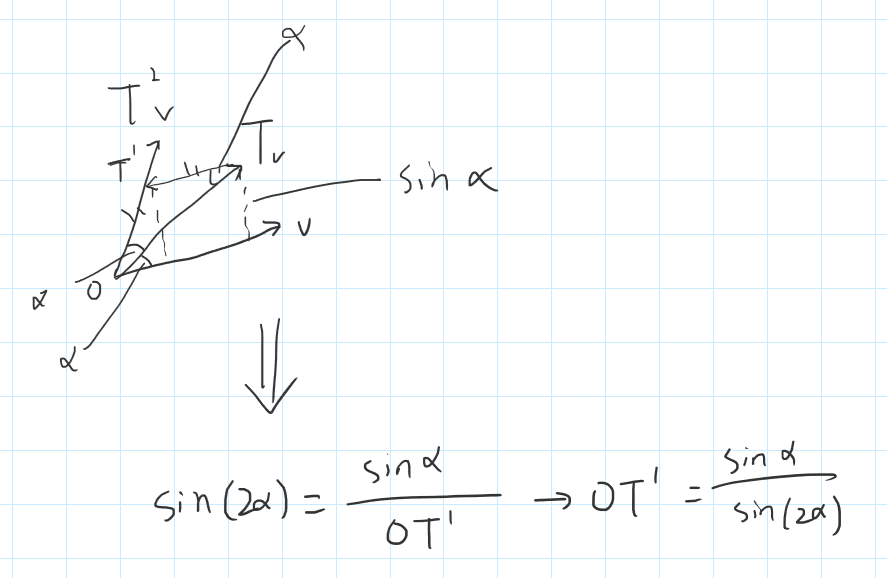
\includegraphics[scale=0.6]{E5B-8-resource}

  $\lambda$ should be $\frac{\sin(1^{\circ})}{\sin(2^\circ)}$, thus
  $p(T) = - \lambda I + T - \lambda T^2$.

  We suppose all $v$ below has length $1$, thus $v = (\cos \theta, \sin \theta)$,
  this doesn't lose the generalizability since $p(T)(\alpha v) = \alpha (p(T)v)$.

  For the first component of $p(T)v = - \lambda v + Tv - \lambda T^2v$, we have:
  \begin{align*}
     & \frac{\sin(1^\circ)}{\sin(2^\circ)} (- \cos \theta - \cos (\theta + 2^\circ)) \\
    =& \frac{\sin(1^\circ)}{\sin(2^\circ)} (- \cos \theta - (\cos \theta \cos(2^\circ) - \sin \theta \sin (2^\circ))) \\
    =& \frac{\sin(1^\circ)}{\sin(2^\circ)} (- \cos \theta - \cos \theta \cos(2^\circ)) + \sin \theta \sin (1^\circ) \\
    =& \cos \theta \frac{\sin(1^\circ)}{\sin(2^\circ)} (- 1 - \cos(2^\circ)) + \sin \theta \sin (1^\circ) \\
  \end{align*}
  where $\sin \theta \sin(1^\circ)$ cancels a part of
  $(Tv)_1 = \cos(\theta + 1^\circ) = \cos \theta \cos (1^\circ) - \sin \theta \sin (1^\circ)$.
  Thus we will show that $\frac{\sin(1^\circ)}{\sin(2^\circ)} (- 1 - \cos(2^\circ)) = - \cos (1^\circ)$.
  \begin{align*}
     & \frac{\sin(1^\circ)}{\sin(2^\circ)} (- 1 - \cos(2^\circ)) \\
    =& \frac{\sin(1^\circ)}{2\sin(1^\circ)\cos(1^\circ)} (- (\cos^2(1^\circ) + \sin^2(1^\circ)) - \cos^2(1^\circ) + \sin^2(1^\circ)) \\
    =& \frac{1}{2\cos(1^\circ)} (- \cos^2(1^\circ) - \cos^2(1^\circ)) \\
    =& \frac{1}{2\cos(1^\circ)} (- 2 \cos^2(1^\circ)) \\
    =& - \cos(1^\circ) \\
  \end{align*}

  For the second component of $p(T)v$, we have:
  \begin{align*}
     & \frac{\sin(1^\circ)}{\sin(2^\circ)} (- \sin \theta - \sin (\theta + 2^\circ)) \\
    =& \frac{\sin(1^\circ)}{\sin(2^\circ)} (- \sin \theta - \sin \theta \cos(2^\circ) - \cos \theta \sin (2^\circ)) \\
    =& \sin \theta \frac{\sin(1^\circ)}{\sin(2^\circ)} (- 1 - \cos(2^\circ)) - \cos \theta \sin (1^\circ) \\
  \end{align*}
  similarly, we have $p(T)v_2 = \sin (\theta + 1^\circ) = \sin \theta \cos (1^\circ) + \cos \theta \sin (1^\circ)$ we will show that $\frac{\sin(1^\circ)}{\sin(2^\circ)} (- 1 - \cos(2^\circ)) = - \cos (1^\circ)$,
  which is proven above.
\end{proof}

\begin{exercise}
  Let $T \in \LT(V)$ such that for some basis of $V$, $\mathcal{M}(T)$ consists of
  rational numbers. Try to explain why the coefficients of the minimal polynomial of $T$
  is rational numbers.
\end{exercise}
\begin{proof}
  I don't know, because $\mathbb{Q}$ is also a field?
\end{proof}

\setcounter{exercise}{10}
\begin{exercise}
  Let $V$ a vector space and $\dim V = 2$ and $T \in \LT(V)$ such that $\mathcal{M}(T)$
  for some basis of $V$ is $\begin{bmatrix}
    a & c \\
    b & d \\
  \end{bmatrix}$.
  Show that:
  \begin{itemize}
    \item $T^2 - (a + d)T + (ad - bc)I = 0$
    \item the minimal polynomial of $T$ is:
          \[
          \begin{cases}
            z - a \quad & \text{if } b = c = 0 \text{ and } a = d \\
            z^2 - (a + d) z + (ad - bc) \quad & \text{otherwise}
          \end{cases}
          \]
  \end{itemize}
\end{exercise}
\begin{proof}
  \def\MT{\begin{bmatrix} a & c \\ b & d \end{bmatrix}}
  ~
  \begin{itemize}
    \item \begin{align*}
             & \mathcal{M}(T^2 - (a + d) T + (ad - bc)I) \\
            =& \MT^2 - (a + d)\MT + (ad - bc)I \\
            =& \begin{bmatrix} 
              a^2 + bc & ac + bd \\
              ab + bd & bc + d^2 \\
            \end{bmatrix} - \begin{bmatrix}
              a^2 + ad & ac + cd \\
              ab + bd & ad + d^2 \\
            \end{bmatrix}
            + \begin{bmatrix}
              ad - bc & 0 \\
              0 & ad - bc \\
            \end{bmatrix}
          \end{align*}
    \item If $b = c = 0$ and $a = d$, then $T$ is a scalar multiple of identity operator,
          thus $T = aI$ and $p(T) = -aI + T = 0$.
          Otherwise, $T^2 - (a + d)T + (ad - bc)I = 0$.
  \end{itemize}
\end{proof}

\end{document}